\section{Open problems in mechanistic interpretability methods and foundations}
\label{sec:open-problems-methods-and-foundations}

One way of thinking about what neural networks do internally is that they learn parameters that implement neural algorithms. These neural algorithms take data as input and, through a series of steps, transform their internal activations to produce an output. Different parts of the network learn different steps in the algorithm; mechanistic interpretability aims to describe the function of different network components. 

Broadly speaking, there are two methodological approaches to achieving this. The first approach, often called `reverse engineering', is to decompose the network into components and then attempt to identify the function of those components (\Cref{subsec:reverse-engineering}). This approach “identifies the roles of network components”. Conversely, the second approach, sometimes referred to as `concept-based interpretability', proposes a set of concepts that might be used by the network and then looks for components that appear to correspond to those concepts (\Cref{subsec:concept-based-interpretability}). This approach thus “identifies network components for given roles”.

In this section, we will examine both approaches (`Reverse engineering' and `Concept-based interpretability') (\Cref{fig:reverse_engineering_vs_concept_based}), discussing their methods and open problems. We will also touch on open problems that cut across either approach, including proceduralizing the mechanistic interpretability pipeline (\Cref{subsec:proceduralizing}) and its uses in automating interpretability research (\Cref{subsec:automation}).

\subsection{Reverse engineering: Identifying the roles of network components}
\label{subsec:reverse-engineering}

\subsubsection{Reverse engineering is necessary because AI and humans use different representations and perform different tasks}
\label{subsubsec:reverse-engineering-necessary}

Large language models produce text that closely resembles human writing, and it is tempting to assume that they generate it through cognitive processes similar to those of human writers\footnote{However, even if this assumption were true, understanding LLMs would remain challenging, as we also lack a mechanistic understanding of the cognitive processes involved in human text creation!}. However, humans and AI models often solve problems in different ways. For example, a model that is only 1\% the size of GPT-3 outperforms humans on next-token prediction tasks \citep{shlegeris2024languagemodelsbetterhumans}. Inversely, even state-of-the-art multimodal LLMs struggle with tasks that a four-year-old could easily master, such as learning causal properties of new objects involving simple lights and shapes \citep{kosoy2023comparingmachineschildrenusing}. An even clearer sign that humans and AI are using different representational processes are cases where humans cannot solve a problem at all, as in the case of predicting a protein structure from sequence \citep{jumper2021highly,lin2023evolutionary}.


Even when both humans and AI exhibit comparable levels of competence on a given task, they may use different heuristics. For example, research shows that image models tend to rely more heavily on textural features (such as recognizing elephants by their hide rather than their shape \citep{geirhos2022imagenettrainedcnnsbiasedtexture}) or rely on dataset correlations (as when identifying fish by the fingers that proud fisherman use to hold them \citep{brendel2019approximatingcnnsbagoflocalfeaturesmodels}) to a greater degree than people do. Even simple algorithmic tasks, like modular addition, which humans might solve with simple carries, were solved by a small transformer model by learning a Fourier transform strategy that researchers only understood in retrospect \citep{nanda2023progressmeasuresgrokkingmechanistic}.

To grasp the potentially alien cognition of these models, we must develop methods to uncover and understand the previously unknown concepts and mechanisms implemented within them. In other words, we must be able to reverse engineer these models \citep{Olah_2022}.

\begin{figure}[!t]
    \centering
    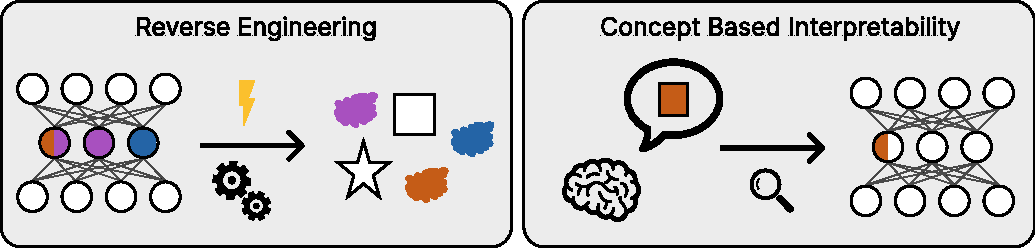
\includegraphics[width=\textwidth]{figures/reverse_engineering_vs_concept_based.pdf}
    \caption{Two approaches to neural network interpretability. (Left) Reverse Engineering is characterized by decomposing networks into functional components and describing how those components interact to produce the network's behavior. It thus aims to `identify the roles of network components' (\Cref{subsec:reverse-engineering}). (Right) Concept-based interpretability on the other hand attempts to discover human concepts within neural network internals. It thus aims to `identify the network components for given roles' (\Cref{subsec:concept-based-interpretability}). 
    }
    \label{fig:reverse_engineering_vs_concept_based}
\end{figure}


Reverse engineering generally involves three steps, whether it is an engine, a piece of software, or a neural network (\Cref{fig:pipeline}):
\begin{enumerate}
    \item \textbf{Decomposition}: Breaking down the object of study into simpler parts (\Cref{subsec:reverse-engineering-step-1});
    \item \textbf{Description of components}: Formulating hypotheses about the functional role of component parts and how they interact (a process that can be called `interpretation') (\Cref{subsec:reverse-engineering-step-2});
    \item \textbf{Validation of descriptions}: Testing if our hypotheses are correct (\Cref{subsec:reverse-engineering-step-3}).
\end{enumerate}

If our hypotheses are invalidated, we must either improve our decomposition or improve our hypotheses regarding the functional roles of its components. We will systematically examine each step, analyzing current methods and their respective shortcomings.

\subsubsection{Reverse engineering step 1: Neural network decomposition}
\label{subsec:reverse-engineering-step-1}

In mechanistic interpretability, our aim is to decompose a neural network and study its parts in isolation in order to explain how neural networks generalize. This aim raises the question of how best to carve a neural network “at its joints” for the purposes of interpretability.

\parasection{Networks do not naturally decompose into architectural components.}
\label{par:decomposition}

The naive approach to decompose neural networks involves breaking them down into their architectural components, such as individual neurons, attention heads, or layers.

Some early attempts to interpret deep artificial neural networks studied the responses or weight structure of individual neurons or single convolutional filters \citep{Erhan_2009_visualising,le2012buildinghighlevelfeaturesusing,Krizhevsky_2012_ImageNet,szegedy2014intriguingpropertiesneuralnetworks,simonyan2014deepinsideconvolutionalnetworks, zhou2015objectdetectorsemergedeep,srivastava_2014,yosinski2015understandingneuralnetworksdeep,Mordvintsev_2015,Olah__2017_FeatureVisualisation,Bau_2017_NetworkDissection,dalvi2018grainsanddesertanalyzing, olah2020an,cammarata2020curve}. These efforts paid homage to the `Neuron Doctrine' in neuroscience, which posits that individual neurons are the structural and functional unit of the nervous system \citep{cajal1924estructura,sherrington1906observations}. However, researchers discovered that single neurons are `polysemantic' -- they seem to respond to multiple kinds of features in both artificial \citep{wei2015understandingintraclassknowledgeinside,nguyen2016multifacetedfeaturevisualizationuncovering,Olah__2017_FeatureVisualisation} and biological networks \citep{churchland2007temporal, rigotti2013importance,mante2013context,raposo2014category}. These observations support earlier theoretical work that suggested representations used by neural networks do not necessarily align with the activation of individual neurons \citep{hinton1981shape}.

Interpreting individual attention heads does not fare better than interpreting individual neurons, as attention heads also exhibit polysemanticity \citep{janiak2023polysemantic}. More broadly, research suggests that studying the attention patterns of models can often be misleading \citep{jain2019attentionexplanation, pruthi2020learningdeceiveattentionbasedexplanations}.

Some work even suggests that representations in language models might span multiple layers \citep{yun2023transformervisualizationdictionarylearning, lindsey2024crosscoders}. This chimes with work that edits or intervenes on individual layers, which indicates that this level is too coarse-grained to robustly carve the network at its joints \citep{meng2022locating,Wang_2022_Circuits}.

If natural architectural components, such as individual neurons, attention heads, or layers, do not provide a natural way to decompose neural network representations, then what does?


\begin{figure}[!t]
    \centering
    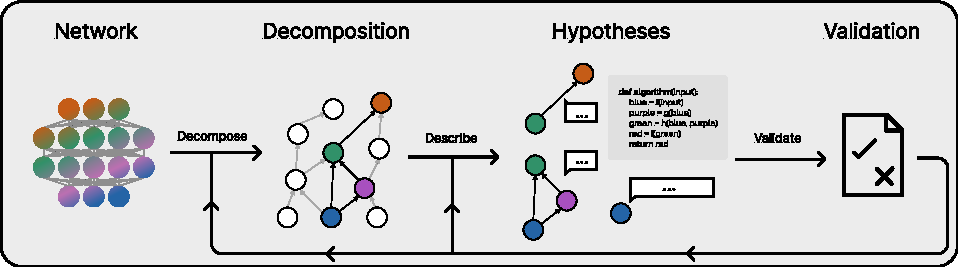
\includegraphics[width=\textwidth]{figures/pipeline.pdf}
    \caption{The steps of reverse engineering neural networks. (1) Decomposing a network into simpler components. This decomposition might not necessarily use architecturally-defined bases, such as individual neurons or layers (\Cref{subsec:reverse-engineering-step-1}). (2) Hypothesizing about the functional roles of some or all components (\Cref{subsec:reverse-engineering-step-2}). (3) Validating whether our hypotheses are correct, creating a cycle in which we iteratively refine our decompositions and hypotheses to improve our understanding of the network (\Cref{subsec:reverse-engineering-step-3}).
    }
    \label{fig:pipeline}
\end{figure}

\parasection{Decomposition by dimensionality reduction methods.}
\label{par:dim-reduction}

If individual neurons are not the right decomposition, perhaps groups or patterns of neurons are. Many decomposition methods attempt to identify activation vectors that correspond to the basic unit of neural network computation. One common approach is to provide models with a range of unlabeled inputs, collect the resulting hidden activations, and then apply unsupervised dimensionality reduction techniques to these hidden activations. The hope is that structure in the hidden activations corresponds to the structure of neural computation. Commonly used dimensionality reduction methods include Principal Component Analysis or Singular Value Decomposition \citep{Tigges_2023_Probe,marks2024geometrytruthemergentlinear,huang2024ravelevaluatinginterpretabilitymethods,bushnaq2024localinteractionbasisidentifying} and non-negative matrix factorization \citep{olah2018the,voss2021visualizing,cammarata2020curve}, though these techniques are no longer predominant methods used for mechanistically decomposing language models \citep{friedman2024interpretabilityillusionsgeneralizationsimplified}.

\parasection{Decomposition by sparse dictionary learning (SDL).}
\label{par:sdl}

According to the `superposition hypothesis', neural networks are capable of representing more features than they have dimensions, as long as each feature activates sparsely \citep{elhage2021mathematical} (\Cref{fig:sdl}). This is a key reason that dimensionality reduction methods are not considered state-of-the-art, because they cannot identify more directions than there are activation dimensions. The superposition hypothesis, coupled with the failure of dimensionality reduction methods to overcome it, motivated the search for methods that can identify more directions than dimensions. Recent work has explored the use of sparse dictionary learning (SDL) to this end \citep{elhage2021mathematical,Sharkey_2022,cunningham2023sparseautoencodershighlyinterpretable,Bricken_2023_dictionary}.

Currently, SDL is the most popular set of unsupervised decomposition methods in mechanistic interpretability. SDL encapsulates a family of methods, including Sparse Autoencoders (SAEs) \citep{gao2024scalingevaluatingsparseautoencoders,templeton2024scaling, rajamanoharan2024improvingdictionarylearninggated, makelov2024principledevaluationssparseautoencoders, kissane2024interpretingattentionlayeroutputs, braun2024identifyingfunctionallyimportantfeatures}, Transcoders \citep{dunefsky2024transcodersinterpretablellmfeature}, and Crosscoders \citep{lindsey2024crosscoders}.


In SDL, hidden activations are typically passed to a small neural network consisting of only two layers, which correspond to an encoder and decoder respectively, with a wide hidden space. The encoder activations represent how active each `latent' \footnote{The term latent is often used instead of the word feature to refer to SDL dictionary elements, since the term `feature' is often used to refer to multiple different ideas \citep{smith2024latent}} is, and the decoder matrix corresponds to a dictionary of latent directions. We want to train the dictionary elements to align with `feature directions' in the network's hidden activations. Since we assume that individual features are sparsely present in the activations, the encoder activations are trained to be sparsely activating. In the case of SAEs, the output is trained to either reconstruct the input or, in the case of transcoders \citep{dunefsky2024transcodersinterpretablellmfeature}, to reconstruct the activations of the next layer. Crosscoders \citep{lindsey2024crosscoders} permit a wider class of inputs and outputs, potentially reconstructing the activations of many layers simultaneously. Since the encoder is nonlinear, it is thought to be able to learn to activate a latent only if a feature is `active' in the hidden activations and remain `off' if it is not.

\begin{figure}[!t]
    \centering
    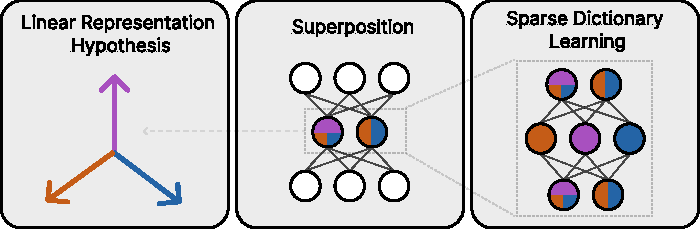
\includegraphics[width=0.8\textwidth]{figures/lrh_etc.pdf}
    \caption{Three ideas underlying the sparse dictionary learning (SDL) paradigm in mechanistic interpretability. (Left) The linear representation hypothesis states that the map from `concepts' to neural activations is linear. (Middle) Superposition is the hypothesis that models represent many more concepts than they have dimensions by representing them both sparsely and linearly in activation spaces. (Right) SDL attempts to recover an overcomplete basis of concepts represented in superposition in activation space.
    }
    \label{fig:sdl}
\end{figure}

Although SDL is considered a leading decomposition method for mechanistic interpretability, it has substantial practical and conceptual limitations (\Cref{fig:sdl-problems}).

\textbf{SDL reconstruction errors are too high}: Large errors in SDL reconstruction raise the question whether SDL methods can reconstruct the hidden representation sufficiently well such that the latents learned by SDL are adequately faithful to the models being interpreted. To measure this, the model's true hidden activations can be replaced with sparse dictionary reconstructions, then subsequently evaluating the extent to which the model's performance decreases. In practice, the error results in significant performance reductions. When a sparse dictionary with 16 million latents was inserted into GPT-4, the language modeling loss was equivalent to a model with only 10\% of GPT-4's pretraining compute \citep{gao2024scalingevaluatingsparseautoencoders}. Similarly, \citet{makelov2024principledevaluationssparseautoencoders} found that using reconstructions from sparse autoencoders decreased GPT-2 small performance by 10\% when trained on task-specific data, and 40\% when trained on the full distribution.

Making sparse dictionaries much larger and sparser to reduce errors is a feasible but computationally expensive approach. Furthermore, in the limit, this results in merely assigning one dictionary latent per datapoint, which is clearly less interpretable. One partial solution is using SDL methods with `error nodes' \citep{marks2024sparsefeaturecircuitsdiscovering}, to account for the discrepancies between the original and reconstructed activations. However, while the sparse autoencoders identified interpretable latents, the error nodes contain `everything else', making them an inadequate solution to the problem. \citet{engels2024decomposingdarkmattersparse} found that these reconstruction errors are not purely random, as much of the direction of the error and its norm can be linearly predicted from the initial activation vector. This suggests that current SDL methods may systematically fail to capture certain structured aspects of model representations, but also implies potential solutions. To overcome this issue, it may be necessary to improve SDL training methods, or develop entirely new methods of network decomposition.

\textbf{SDL methods are expensive to apply to large models}: SDL involves training a small neural network for every layer of the AI model that we want to interpret. Typically, the sparse dictionaries have more parameters at that layer than the original model does, and consequently will probably be relatively expensive to train compared to the original model. \footnote{The actual relative cost is unclear since there are no public attempts to apply SDL to every vector space in a model, although some work applies SDL to various layers \citep{marks2024sparsefeaturecircuitsdiscovering,gao2024scalingevaluatingsparseautoencoders,braun2024identifyingfunctionallyimportantfeatures,lieberum2024gemmascopeopensparse, Bloom_Lin_2024,cunningham2023sparseautoencodershighlyinterpretable}} As AI models become larger, scaling costs of SDL also increase, although it remains unclear whether relative scaling costs are sub- or supra-linear. For cost effectiveness, it may be important to develop intrinsically decomposable methods for training models, while remaining at (or close to) state-of-the-art performance (\Cref{par:intrinsic-interpretability}). This approach will help avoid incurring the expense of both training and decomposing AI models.

\begin{figure}[!t]
    \centering
    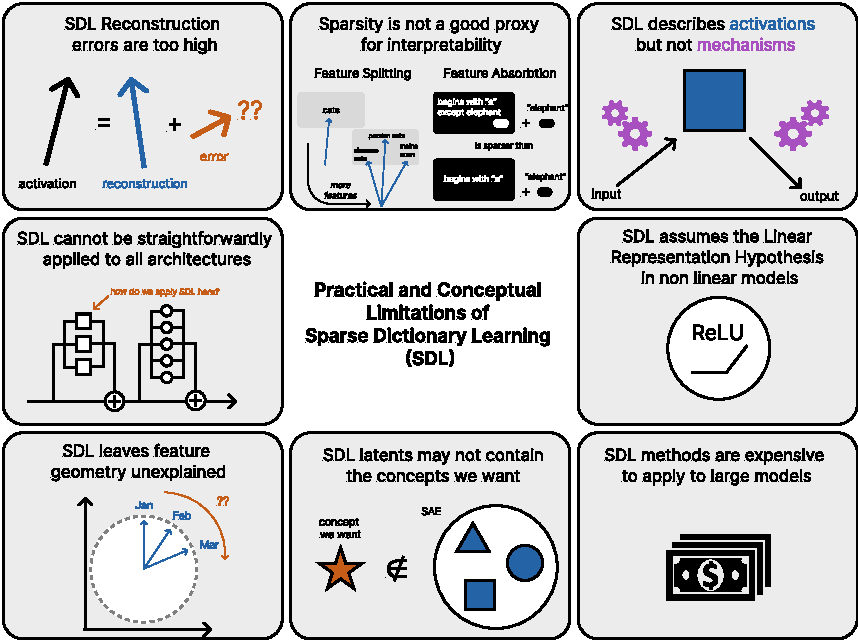
\includegraphics[width=\textwidth]{figures/sdl.pdf}
    \caption{Sparse dictionary learning has a number of practical and conceptual limitations that cause issues when using it to reverse engineer neural networks (\Cref{par:sdl}).}
    \label{fig:sdl-problems}
\end{figure}


\textbf{SDL assumes the linear representation hypothesis in nonlinear models}: Other problems with SDL arise from the assumptions on which SDL is based. One such assumption is the linear representation hypothesis. The linear representation hypothesis observes that though neural networks are nonlinear functions and could potentially use highly nonlinear representations \citep{black2022interpretingneuralnetworkspolytope,engels2024decomposingdarkmattersparse, kirch2024featurespromptsjailbreakllms}, they tend to use representations that exhibit strikingly linear behavior \citep{Smolensky_1986, mikolov-etal-2013-linguistic,olah2020zoom,elhage2021mathematical,park2024linearrepresentationhypothesisgeometry, guerner2024geometricnotioncausalprobing,gurnee2024languagemodelsrepresentspace}. The hypothesis formalizes this phenomenon by stating that high level concepts are linearly represented as directions (vectors) in neural network embeddings. Its two core claims are (i) that the composition of multiple concepts can be represented as the addition of their corresponding feature vectors, and (ii) that the intensity of a concept is represented by the scale of its corresponding feature vector \citep{olah2024linear}. Earlier work \citep{elhage2021mathematical} defined the linear representation hypothesis with the additional assumption of one-dimensional features, but this definition has since been refuted \citep{Yedidia_2023,chughtai2024understanding, engels2024languagemodelfeatureslinear} and clarified \citep{olah2024linear}. Another recently proposed criterion is that the intensity of concepts should be retrievable by a linear function of the embeddings, up to a small error \citep{hani2024mathematicalmodels, olah2024linear}.

A weak version of the linear representation hypothesis states that some concepts are linearly represented, while a strong version may assert that all concepts are \citep{Smith_2024_strongfeature}. Some works have shown that the strong version is false for some models \citep{black2022interpretingneuralnetworkspolytope, csordás2024recurrentneuralnetworkslearn}. The weaker version of the linear representation hypothesis is supported by the successes of linear probes (\Cref{subsubsec:concept-based-probes}), activation steering (\Cref{subsec:better-control}), and the success of sparse autoencoders in finding seemingly interpretable latents (\Cref{par:sdl}).

\textbf{Sparsity is not a good proxy for interpretability}: Another of SDL's key assumptions is that feature activations are sparse. Therefore, SDL methods optimize their latents accordingly to be sparsely activating, with the implicit assumption that sparser decompositions are more interpretable than denser ones. However, this assumption may not necessarily hold. The (related) problems of feature splitting \citep{Bricken_2023_dictionary}, feature absorption \citep{chanin2024absorptionstudyingfeaturesplitting} and composition \citep{till2024sparse} suggest that with sufficient optimization pressure, sparsity as a proxy for interpretability breaks down (though note that it is debated whether feature splitting is actually a problem). Other proxies, such as minimum description length, might be better optimization targets than sparsity \textit{per se} \citep{ayonrinde2024interpretabilitycompressionreconsideringsae}. It also may be the case that no proxy metric is sufficient.

\textbf{SDL leaves feature geometry unexplained}: SDL decomposes networks into single directions in the activation space, which is a reasonable approach only if we consider feature activations akin to `a bag of features' \citep{Harris_1954_distributionalstructure} without any internal structure. However, the geometric arrangement of features in relation to each other seems to reflect semantic and functional structure \citep{engels2024languagemodelfeatureslinear,gurnee2024languagemodelsrepresentspace, park2024geometrycategoricalhierarchicalconcepts,bussman2024metasaes}. Understanding the geometric structure of a network means understanding the position of one feature relative to (potentially) many others. Comprehending this may be necessary if we want to know why and how a network treats certain features similarly or differently. If understanding the global geometry (all-to-all relationships) of features is essential to understand neural networks, this might pose a fundamental problem for current approaches to mechanistic interpretability \citep{hani2024mathematicalmodels, mendel2024sae}. However, if only local geometric relationships between features need to be understood, understanding networks with a `bag of features' approach may be more feasible.

\textbf{SDL cannot straightforwardly be applied to all architectures}: SDL was originally developed to identify features that may be represented in superposition across many neurons within a single layer. However, representations may be spread over other network architecture components besides neurons. In transformers, for example, representations may be spread across separate attention heads \citep{jermyn2023attention, janiak2023polysemantic}, and even across different layers \citep{yun2023transformervisualizationdictionarylearning, lindsey2024crosscoders}. However, it is not immediately obvious how to decompose representations distributed across attention heads with SDL \citep{mathwin2024gated, wynroe2024decomposing}. Nor is it straightforward to translate cross-layer distributed representations into causal descriptions of neural network mechanisms \citep{lindsey2024crosscoders}.

\textbf{SDL decomposes the input and output activations of network mechanisms, but not the mechanisms themselves}: Ultimately, the aim of mechanistic interpretability is to understand the mechanisms learned by neural networks. The parameters of the network, along with its nonlinearities and other architectural components, implement these mechanisms, which are applied to the input's hidden activations. SDL identifies directions in activation space. Being activations, they only interact with the network's mechanisms, but are not the mechanisms themselves. Describing the mechanisms directly remains unresolved with SDL. Gaining insights about the network's mechanisms from SDL latents requires further post hoc analysis, which can be labor intensive, computationally expensive, or data set dependent \citep{cunningham2023sparseautoencodershighlyinterpretable,Bricken_2023_dictionary, riggs2023finding,marks2024sparsefeaturecircuitsdiscovering}. This is an instance of a more broad problem with current mechanistic interpretability work; we primarily focus on understanding neural network activations, with little attention paid to how this structure in activations is computed via weights \citep{chughtai2025activation}.


\textbf{SDL latents may not contain the concepts needed for downstream use cases}: When using SAEs for practical tasks, there sometimes exists a single latent or small set of latents representing some concept of interest for task performance (and not representing much else). For instance, \citet{kantamneni2024sae} found a single latent whose activation pattern was more accurate than official dataset labels on the NLP task GLUE CoLA \citep{warstadt2019neuralnetworkacceptabilityjudgments}. More often than not though, a sparse set of latents that encode some useful concept of interest do not exist. It is unclear what causes this problem. One hypothesis is that the concept we want isn't how the model `thinks' about the concept, and the SAE is working as intended. Alternatively, the SAE training distribution could be too narrow, resulting in the SAE not being incentivised to learn the important latents. \citep{kissane2024saes} found that SAEs trained on pretraining data generally do not have good latents for the concept of `refusing' harmful user requests, while SAEs trained on chat formatted data do. Or, the SAE might not have a large enough dictionary size to learn all concepts of interest. Many more hypotheses are plausible. A complicating factor in using SDL to identify the learned mechanisms of neural networks is that the latents identified by depend on the data set used to train them. This is an undesirable property for a decomposition method that was initially hoped to be capable of identifying the fundamental units of computation in neural networks \citep{kissane2024saes}.


\parasection{Current decomposition methods lack solid theoretical foundations.}
\label{par:theoretical-foundations}

Given the practical and conceptual issues with SDL, there is broad agreement that the question of how to correctly decompose networks into atomic units remains a central problem, evidenced by the large amount of effort focused on the direction in recent years. After investing considerable effort in SDL approaches, it is apparent that improved conceptual clarity beyond the idea of superposition \citep{elhage2021mathematical} is needed to advance neural network decomposition.

One of the most significant open questions is the absence of clarity around the nature of features, despite being the central focus of SDL's identification efforts. Satisfying formal definitions are elusive and conceptual foundations are not yet established. However, even without foundations, progress in mechanistic interpretability is possible — even confused concepts can be pragmatically useful \citep{henighan2024caloric}.

Without solid conceptual foundations, it remains unclear whether the superposition hypothesis, which underpins the SDL paradigm, is fundamentally valid or merely pragmatically useful \citep{henighan2024caloric,templeton2024scaling}. If it is the latter, there may be better methods than SDL for carving neural networks at their joints. Such methods may take into account feature geometry or take a more dynamic, developmental view of how mechanistic structure emerges in the training process \citep{hoogland2024developmentallandscapeincontextlearning, wang2024loss}. Moreover, although there is much emphasis on how models represent features in superposition, there is comparatively less work examining how they might perform computation on them natively in superposition. Further conceptual work into this problem may suggest new methodologies for decomposing networks, or provide bounds on the number of features we should expect models to be capable of learning \citep{hani2024mathematicalmodels, adler2024complexityneuralcomputationsuperposition, bushnaq2024circuits}.

Mechanistic interpretability should ideally be built on more formal foundations. Some work attempts to ground mechanistic interpretability in the formalisms of causality \citep{Geiger_2023_CausalAbstractionRepresentationSubspace}. However, this approach has not yet yielded canonical causal mediators \citep{mueller2024questrightmediatorhistory} that may form a basis for decomposition methods. How should we go about finding them? Given that our field's objective is to understand the learned structures that underlie networks' generalization behaviors, exploring theories about why neural networks generalize appears to be a promising avenue. But theories that attempt to characterize why neural networks generalize, such as the spline theory of neural networks \citep{balestriero_2018_spline}, theories of neural networks' simplicity bias \citep{vallepérez2019deeplearninggeneralizesparameterfunction}, deep learning theory involving the neural tangent kernel \citep{jacot2020neuraltangentkernelconvergence,Roberts_2022_principles}, or singular learning theory \citep{Watanabe_2009, Wei_2023_deeplearningsingular} have either not yet yielded mathematical objects that can be easily used for interpretability, or simply have not been successfully linked to approaches for interpreting neural networks. Establishing these connections would make significant progress toward carving neural networks at their joints to facilitate mechanistic interpretability. And if we can carve trained networks at their joints, it may suggest ways to train networks such that they come `pre-carved'. Thus, better theoretical foundations may also be important for developing models that are intrinsically decomposable by design, which we discuss next.

\parasection{Intrinsic interpretability: Building more easily decomposable models}
\label{par:intrinsic-interpretability}

The current strategy of training a model solely for performance and then interpreting it post hoc may not be optimal if our goal is a model that is both interpretable and performant. To this end, it may be beneficial to prioritize interpretability during model training, for which there are several plausible approaches. 

Instead of post-hoc decomposing trained network activations into discrete codes (\Cref{par:sdl}), network activations could be forced to use a discrete code from the outset, as in \citet{tamkin2023codebookfeaturessparsediscrete}. MLPs could also be trained with sparser activation functions, such as TopK \citep{makhzani2013ksparseautoencoders,bills2023language} or SoLU \citep{elhage2022solu}. Similar approaches could be potentially used to restrict attention superposition \citep{jermyn2023attention} by limiting the number of heads attending to any query-key pair. Several approaches, such as `mixture of experts' \citep{shazeer2017outrageouslylargeneuralnetworks,switchtransformers, he2024mixturemillionexperts}, use sparsely activating components — with a large enough number of experts, and with sufficient activation sparsity, experts may become individually interpretable \citep{warstadt2019neuralnetworkacceptabilityjudgments}. Many attempts to incentivize interpretable activations directly so far have not been competitively performant, and have also allowed `superposition to sneak through', mitigating benefits.

We can also target weight sparsity directly during training, including approaches such as L0 regularization \citep{louizos2018learningsparseneuralnetworks} or pruning \citep{Mozer_1988_skeletonization,frankle2019lotterytickethypothesisfinding, mocanu2018scalable}. \citet{Han_2015_weightsandconnections} achieve sparse weights by using magnitude pruning followed by finetuning. This highlights a general strategy of finetuning with interpretability in mind (also used by \citet{tamkin2023codebookfeaturessparsediscrete}), avoiding the potentially excessive cost of training from scratch. Another related strategy is targeting modularity \citep{Kirsch_2018_modularnetworks, andreas2017neuralmodulenetworks}. For example, brain-inspired modular training \citep{liu2023seeingbelievingbraininspiredmodular} trains for modularity by embedding neurons in a geometric space and encouraging geometrically local connections.

Existing research implements other approaches that can simplify linearity-reliant circuit analysis \citep{elhage2021mathematical}. For example, there is work removing the layer norm operations \citep{heimersheim2024removegpt2slayernormfinetuning}, using input-switched affine transformations for recurrence \citep{foerster2017inputswitchedaffinenetworks}. Other studies leverage architectures that are mathematically analyzable in other ways than linearity, such bilinear activations in MLPs \citep{sharkey2023technicalnotebilinearlayers, pearce2024weightbaseddecompositioncasebilinear}.

After decomposing a network into components, whether through post hoc decomposition or by using intrinsically decomposable models, our task remains unfinished. We must provide an interpretation of the functional role of each component (Step 2 -- \Cref{subsec:reverse-engineering-step-2}) and validate that interpretation (Step 3 -- \Cref{subsec:reverse-engineering-step-3}). In the next section, we will discuss common methods of interpretation and their shortcomings.


\subsubsection{Reverse engineering step 2: Describing the functional role of components}
\label{subsec:reverse-engineering-step-2}

After decomposing networks into parts, the next step of reverse engineering is to “describe” the functional role of these components. This step is best thought of as generating hypothesized `interpretations' or `explanations'. These explanations form candidate descriptions of the functional role of a given component, and should not be taken to be definitive conclusions before they are thoroughly validated (see \Cref{subsec:reverse-engineering-step-3}).

Descriptions of the functional role of neural network components can either indicate (1) the cause of a component's activation or (2) what occurs after that component has been activated, or -- preferably -- both (\Cref{fig:descriptions}). In this section, we will discuss the existing set of tools available to mechanistic interpretability researchers to describe the functional role of network components.

\begin{figure}[h]
    \centering
    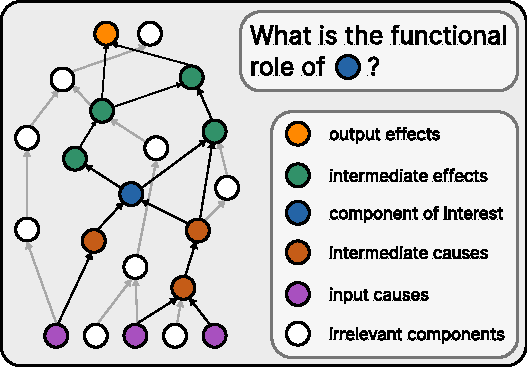
\includegraphics[width=0.6\textwidth]{figures/descriptions.pdf}
    \caption{To study the functional role of \textcolor{NavyBlue}{the blue component} numerous approaches are possible. We could study its causes: \textcolor{Purple}{the purple input components} or \textcolor{Bittersweet}{the red intermediate components} via e.g. feature synthesis \citep{Olah__2017_FeatureVisualisation, olah2020zoom}, maximum activating examples \citep{Olah__2017_FeatureVisualisation, Bricken_2023_dictionary}, or attributions \citep{Sundarajan_2017_IntegratedGradients}. Or we could study its effects: \textcolor{orange}{the orange output components} or \textcolor{OliveGreen}{the green intermediate components} via e.g. the logit lens \citep{Nostalgebraist_2020}, activation steering \citep{turner2024steeringlanguagemodelsactivation}, or attributions \citep{marks2024sparsefeaturecircuitsdiscovering}.}
    \label{fig:descriptions}
\end{figure}



\parasection{Explanations for what causes components to activate}
\label{par:activation-causes}

Explanations of the causes of component activation can use three broad categories of methods, each with several problems: (1) Highly activating data set examples; (2) Attribution methods; and (3) Feature synthesis.

\textbf{Highly activating data set examples}. The simplest method is to use highly activating data set examples (sometimes called `exemplar representations' \citep{hernandez2022natural}). These are inputs on which a particular component is strongly activated. For a given component, analyzing apparent commonalities in the inputs suggests hypotheses for what causes that component to activate. This step may be carried out by humans or AI systems (\Cref{subsec:automation}).

Despite being widely used, this approach has several substantial issues. The first issue is that the method relies on human prior beliefs, which may lead interpreters to project their human understanding onto models that may, in fact, be using unfamiliar concepts. This bias could lead us to identify concepts in the model that do not truly explain the mode's functioning \citep{Freiesleben_2023_weneedtotalk, Donnelly_2019_sentimentneuron, GALE_2020_ObjectDetectors}.

Another issue with this approach is the potential for `interpretability illusions'. \citet{bolukbasi2021interpretabilityillusionbert} show that bias in data sets can create misleading explanations even when top activating examples are selected from real data sets, as opposed to synthetically created data. Depending on the data set from which the examples were drawn, human annotators identified dramatically different meanings for given directions in the activation space of BERT \citep{devlin2019bertpretrainingdeepbidirectional}.

A third issue is that this approach often yields plausible explanations for arbitrarily chosen directions in the activation space \citep{szegedy2014intriguingpropertiesneuralnetworks}. This means that plausible explanations based on highly activating data set examples cannot be solely relied upon to identify the basic units of computations in neural networks — other methods are needed to accurately identify them. Furthermore, it is possible to develop adversarial models that deliberately yield misleading feature visualizations \citep{geirhos2024donttrusteyesunreliability}.

Many of the issues with highly activating data set examples stem from the fact that they merely provide correlational explanations for the activation of a network component, rather than causal explanations. To identify causal explanations, other methods, such as attribution methods, are necessary.

\textbf{Attribution methods are necessary for causal explanations but are often difficult to interpret}. Attribution methods \citep{Simonyan_2014_BackpropVisualisation, Nguyen_2016_FeatureVisualization, Selvaraju_2019_GradCAM, Sundarajan_2017_IntegratedGradients, Fong_2017_MaskingBasedCausalAttribution, Lundberg_2017_SHAP,Ribiero_2016_LIME} are intended to measure the causal importance of upstream variables (such as inputs) on downstream variables (such as a network component). They are often gradient-based \citep{Mozer_1988_skeletonization, Simonyan_2014_BackpropVisualisation, Nguyen_2016_FeatureVisualization, Selvaraju_2019_GradCAM, Sundarajan_2017_IntegratedGradients, wang2024gradientbasedfeatureattribution} or sampling-, perturbation-, or ablation-based \citep{Fong_2017_MaskingBasedCausalAttribution, vig2020causalmediationanalysisinterpreting, geiger2020neuralnaturallanguageinference, Ghorbani_2020,meng2022locating, Chan_Garriga-alonso_Goldowsky-Dill_2022,NeelNanda_2023a}. However, on a theoretical level, many gradient-based methods identify only a first-order approximation of the ideal attribution, which is sometimes a poor approximation \citep{watson2022conceptual}. \citet{adebayo2020sanitycheckssaliencymaps} revealed more practical implications, demonstrating that some gradient-based methods identify attributions that are independent both of the model and of the data generating process. Furthermore, an adversary can train a model or perturb an input to reveal any attribution map \citep{Dombrowski_2019_advances, Ghorbani_Abid_Zou_2019, Heo_2019_Advances, Kindermans2019saliencymethods, Slack_2020_foolinglime, zhang2019interpretabledeeplearning}\footnote{However, \citet{Freiesleben_2023_weneedtotalk} argue that adversarial examples do not truly undermine saliency maps as these are highly dissimilar to real interpretability challenges.}. Perturbation methods present certain issues, such as taking models off their training distribution and eliciting unusual behavior, among other theoretical complications \citep{feng-etal-2018-pathologies, molnar2021generalpitfallsmodelagnosticinterpretation, hooker2021unrestrictedpermutationforcesextrapolation, molnar2024model, Freiesleben_2023_weneedtotalk, Slac_2021_advances}. Developing efficient and accurate attribution methods thus remains an open problem.

\textbf{Feature synthesis}. Feature synthesis is a strategy that combines highly activating data set examples and gradient-based attribution methods 
\citep{Erhan_2009_visualising, szegedy2014intriguingpropertiesneuralnetworks,Olah__2017_FeatureVisualisation}. This approach attempts to synthesize inputs that maximize the activation of a component subject to some regularization, such as consistency with a generative model \citep{nguyen2016synthesizingpreferredinputsneurons, nguyen2017plugplaygenerative} or total variation distance \citep{mahendran2014understandingdeepimagerepresentations}. However, criticisms of feature synthesis methods suggest that natural dataset examples may serve interpretation better \citep{zimmermann2021how, borowski2021exemplarynaturalimagesexplain} or show that current methods struggle to identify trojans \citep{casper2023redteamingdeepneural}.

\parasection{Explanations for the downstream effects of components}
\label{par:downstream-effects}

Alternatively, the functional role of a component can be described through its downstream effects.

\textbf{Studying the direct effect}. The logit lens \citep{Nostalgebraist_2020} applies the models unembedding matrix to an intermediate residual stream representations, converting it into a distribution over the model's output vocabulary. Direct logit attribution is a generalization of this technique, applying to any appropriately sized vector space in the model, e.g. the output of MLP layers \citep{geva2021transformerfeedforwardlayerskeyvalue,geva2022transformerfeedforwardlayersbuild,geva2022lmdebuggerinteractivetoolinspection,dar-etal-2023-analyzing}, attention blocks, gradients \citep{katz2024backwardlensprojectinglanguage} of these, and SDL decoder weights \citep{Bricken_2023_dictionary}. Adding a trainable affine or linear transformation before unembedding, as also referred to as the tuned lens, improves decoding accuracy \citep{belrose2023elicitinglatentpredictionstransformers,yom-din-etal-2024-jump}, at the cost of less faithfully representing when the model has completed computation.

In the language of causality \citep{Pearl_2009}, unembedding a residual stream vector measures the direct effect of that vector on the output \citep{mcgrath2023hydraeffectemergentselfrepair}. However, the logit lens cannot measure the indirect effect, the effects resulting from the influence that the embedding has on the hidden activations of subsequent layers. Other methods, such as causal interventions (see below), are necessary to measure the indirect effect. In the future, it may be possible to extend logit-lens-like approaches to not only project the effects of network components on directions in output vocabulary space, but also on intermediate downstream components.

\textbf{Causal Interventions}. Causal interventions typically substitute (“patch”) the value of some network component, usually an activation vector, with a different value during a forward pass, observing the resulting effect on the model. There exist a related set of techniques: ablation (for the special case of zero-ing or otherwise attempting to delete activations entirely), activation patching, causal mediation analysis, causal tracing, and interchange intervention \citep{vig2020causalmediationanalysisinterpreting, geiger2020neuralnaturallanguageinference, meng2023locatingeditingfactualassociations, Chan_Garriga-alonso_Goldowsky-Dill_2022, NeelNanda_2023a}. \footnote{For instance, by patching activations from the corrupt prompt “the capital of Italy is” into the clean prompt “the capital of France is”, we can observe the effect on the output (“Rome” vs.“Paris”). This tells us which component values are relevant for the differing output between the two prompts, but not the information that remains consistent (e.g. the fact that the answer is a city).}

More surgical patches are also sometimes also made on edges between network components. This approach, known as “path” patching, allows us to isolate the effect of one particular component on only one other component, instead of on the entire rest of the network \citep{goldowskydill2023localizingmodelbehaviorpath}. Causal scrubbing \citep{Chan_Garriga-alonso_Goldowsky-Dill_2022} is a generalization of path patching that allows for testing hypotheses concerning any given connection between a set of network components.

Causal intervention methods can also generate supervision signal to identify subspaces of interest. For instance, distributed alignment search \citep{geiger2024findingalignmentsinterpretablecausal} learns a linear subspace that represents a particular concept, using data with interventions on that concept as supervision \citep{geiger2024findingalignmentsinterpretablecausal, guerner2024geometricnotioncausalprobing, wu2024interpretabilityscaleidentifyingcausal}. Other work learns masks over network components to remove irrelevant components \citep{de-cao-etal-2020-decisions, csordás2021neuralnetsmodularinspecting, davies2023discoveringvariablebindingcircuitry}.

A causal intervention typically requires a forward pass of the model. This may make performing one for every network component in large models, long contexts, or when using finer-grained components such as sparse autoencoder latents prohibitively expensive. Faster alternatives that work well in practice \citep{marks2024sparsefeaturecircuitsdiscovering,templeton2024scaling} include gradient-based approximations to activation patching, such as attribution patching \citep{NeelNanda_2023a, syed2023attributionpatchingoutperformsautomated}, AtP* \citep{kramár2024atpefficientscalablemethod}, and integrated gradients \citep{Sundarajan_2017_IntegratedGradients}.

\textbf{Observing the effects of components on sequential behavior}. Another way to study the effects of model components is to patch in activated components and observe their effect on model behavior. Steering is one example of this \citep{panickssery2024steeringllama2contrastive,turner2024steeringlanguagemodelsactivation}, where components (activation vectors) are activated in order to influence the network's behavior, often in interpretable ways. To determine the functional role of an activation vector, a related method is to have a language model itself decode the activations \citep{chen2024selfieselfinterpretationlargelanguage, Mwatkins_2023, ghandeharioun2024patchscopesunifyingframeworkinspecting, huang2024inversionviewgeneralpurposemethodreading, kharlapenko2024self}. These approaches, known as “patchscopes”, patch activations from one forward pass of a model into a different forward pass (perhaps in a different model). The context of the new forward pass is designed to elicit relevant information from the activations of the original forward pass.

A related sequential behavior based technique is simply to read the chain-of-thought \citep{wei2023chainofthoughtpromptingelicitsreasoning, kojima2023largelanguagemodelszeroshot} produced by a language model's output. While this could be considered an `interpretability technique' in the sense that it aims to explain model decisions, it does not use model internals in those explanations, at least not directly. Recent research demonstrates that chains of thought are not entirely faithful to the model's underlying decision-making process \citep{agarwal2024faithfulnessvsplausibilityunreliability, atanasova2023faithfulnesstestsnaturallanguage, Turpin2023_cot, lanham2023measuringfaithfulnesschainofthoughtreasoning, Ye_2022_unreliability}. A promising future direction for interpretability research may be to incorporate model internals into chain-of-thought training, which could incentivize faithfulness. Another possibility is building monitors based on model internals to improve transparency in chain-of-thought faithfulness.

\subsubsection{Reverse engineering step 3: Validation of descriptions}
\label{subsec:reverse-engineering-step-3}

Initial descriptions of network components' functional roles should be treated as hypotheses that first require validation to ensure that they are reasonable.

Conflating hypotheses with conclusions has regrettably been commonplace in mechanistic interpretability research, making validation an important area for the field to improve \citep{madsen2024interpretabilityneedsnewparadigm, stander2024grokkinggroupmultiplicationcosets}. Unfortunately, it is often hard to distinguish faithful explanations of neural network components from merely plausible ones. Numerous examples of model interpretations fail sanity checks \citep{adebayo2020sanitycheckssaliencymaps, leavitt2020falsifiableinterpretabilityresearch, miller2024transformercircuitfaithfulnessmetrics}; “interpretability illusions” in which seemingly convincing interpretations of a model later turned out to be false \citep{bolukbasi2021interpretabilityillusionbert,makelov2023subspacelookingforinterpretability}; or instances where different approaches to explaining the same phenomenon yielded different interpretations (e.g. \citet{Chan_2022_InductionHeads} or \citet{chughtai_2023_toyModel} vs. \citet{stander2024grokkinggroupmultiplicationcosets} vs.  \citet{wu2024unifyingverifyingmechanisticinterpretations}). Several other instances were previously cited in this review (\Cref{subsec:reverse-engineering-step-2}). Hypotheses in interpretability require extensive validation beyond what appearances might imply.

Validating a hypothesis involves posing a simple question: Does the hypothesis make good predictions about the neural network's behavior? Testing the hypothesis often requires multiple approaches \citep{mueller2024questrightmediatorhistory}. To validate descriptions, many approaches simply apply a different description method than the one used to generate the initial hypothesis (\Cref{subsec:reverse-engineering-step-2}). If one description method yields a different description from another, it invalidates the hypothesis, which necessitates returning to an earlier step in the reverse engineering cycle (\Cref{fig:pipeline}). However, methods for validating descriptions are not limited to other component description methods. Hypothesis validation may take many forms, including the following:

\textbf{Predicting activations and counterfactuals}: By using natural language explanations of a given network component's function, it is possible to predict the component's activation levels on different inputs. This analysis can be carried out by humans or by AI systems (\Cref{subsec:automation}), as in \citep{hernandez2022natural,bills2023language,shaham2024multimodalautomatedinterpretabilityagent, Belrose_2024_autointerp}. In essence, our interpretations should enable us to successfully predict counterfactual scenarios in neural networks. For instance, if we ablate or activate particular network components, we should be able to predict specific downstream effects on other components.

\textbf{Predicting and explaining unusual failures or adversarial examples}: Good explanations of neural network behavior should help us identify and explain cases where that behavior fails to produce expected outcomes. For instance, \citet{hilton2020understanding} validated their methods by explaining cases where a deep reinforcement learning agent's neural network failed to achieve maximum reward and also explained specific hallucinations exhibited by the network. Another approach is to use use an interpretability approach to handcraft an input for a network that functioned as an adversarial example \citep{carter2019activation, casper2023diagnosticsdeepneuralnetworks, Mu_2020_Advances, hernandez2022natural}.

\textbf{Handcrafting a network that reconstructs a network behavior}: If our explanations for network behavior are sufficient, we should be able to use them to build replacement parts for the original network. \citet{cammarata2020curve} validated their interpretation of a curve detector's function in a convolutional neural network by substituting its parts with simple handcrafted replacements.

\textbf{Testing on ground truth}: If the weights of a toy neural network were handcrafted by humans, it is possible to obtain a ground truth explanation for how it works. This proves useful for testing explanations produced by interpretability methods. For example, \citet{conmy2023automatedcircuitdiscoverymechanistic} validated a tool's ability to attribute model behaviors to internal components by running it on a simple model that implemented a known algorithm. (See also \Cref{par:benchmarks}).

\textbf{Using the hypothesis to achieve particular engineering goals}: 
Another way to test explanations is to assess their utility in downstream applications \citep{doshivelez2017rigorousscienceinterpretablemachine, casper2023redteamingdeepneural}. For example, \citet{templeton2024scaling} discussed examples where manually editing a large language model based on an interpretation led to predictable high-level changes in its behavior. Meanwhile, \cite{marks2024sparsefeaturecircuitsdiscovering} showed how an interpretability tool could assist humans with debugging a classifier in a toy task. \citet{farrell2024applyingsparseautoencodersunlearn} use unlearning (\Cref{subsec:better-control}) to demonstrate that learned SDL latents don't quite match human concepts, and might not be optimal for particular downstream use cases, highlighting potential issues with SDL.

\textbf{Using the hypothesis to achieve specific engineering goals competitively}: Achieving not only useful, but competitive methods sets an even higher standard. For interpretability tools, the highest evaluation criteria require fair comparisons against relevant baselines on real-world tasks instead of cherry-picking them. However, the practice of conducting evaluations using non-cherry-picked tasks remains relatively uncommon. Although attempts have been made to use techniques in the current interpretability toolkit in such evaluations, they have not proven to be consistently useful \citep{adebayo2020debuggingtestsmodelexplanations,denain2023auditingvisualizationstransparencymethods,Caspar_2023_RedTeamingDNNFeatureSynthesis,hase2023doeslocalizationinformediting, durmus2024steering}. Some of the most promising research directions are to use interpretability methods to achieve things that would be hard or impossible to achieve without them \citep{schut2023bridginghumanaiknowledgegap}. Unless interpretability methods demonstrate that they are competitive with alternative approaches to achieve engineering goals, then the act of demonstrating their usefulness may lead to a bias toward developing methods that only perform well in best-case scenarios and on simple tasks, rather than those that can handle worst-case scenarios and practical challenges.

Interpretability researchers have historically faced challenges in adequately validating their hypotheses due to the high costs in terms of time and cognitive labor. In the following section, we explore two potential solutions that could simplify the validation process: model organisms and interpretability benchmarks.

\parasection{`Model organisms' facilitate hypothesis validation.}
\label{par:model-organisms}

Although interpretability is sometimes motivated by achieving engineering goals, it is often also approached through the perspective of the natural sciences \citep{olah2020zoom}. In certain natural sciences, such as genomics and neuroscience, it is common for researchers to investigate a few extensively studied species known as `model organisms' or 'model systems'. By conducting in-depth studies on a select group of organisms, like \textit{E. coli}, fruit flies, mice, and macaque monkeys, researchers can leverage the insights and tools gained from those organisms and apply them to other species. For example, imaging specific types of neural activity in mice is more tractable due to existing hypotheses about which proteins should be fluorescently labeled in order to identify specific types of neurons. The use of model organisms allows for cross-checking results with previous work, enabling stronger validation of hypotheses.

Currently, interpretability researchers lack consensus on which networks should serve as model organisms. Essentially, what should the \textit{Drosophila melanogaster} of mechanistic interpretability be? In mechanistic interpretability, an ideal model organism should be open source, easy and cheap to use, representative of a broad range of systems and phenomena, have a replicable training process with open source training data, and have multiple instances with different random seeds, among other criteria \citep{Sharkey_2022_CurrentThemes}. Thus far, researchers have mostly used model organisms that possess only some of these criteria, such as a transformer than can perform modular addition \citep{nanda2023progressmeasuresgrokkingmechanistic} or GPT-2 \citep{radford2018language}.

Model organisms not only support cross-validation of hypotheses, but also facilitate the progressive construction of experimental infrastructure by providing a reliable foundation for experiment design. This simplifies the process of rigorous hypothesis testing, thus helping prevent oversimplification and `interpretability illusions'.

Studying solely model organisms, instead of more directly pursuing engineering goals, risks merely making true statements about neural network structure, rather generating insights that are of immediate practical benefit. For mechanistic interpretability to make the fastest and most substantial progress toward engineering goals, both scientific and engineering wins should be pursued in parallel.

Furthermore, certain choices made while studying model organisms risk steering the field in suboptimal directions. For instance, interpretability research is often motivated by the engineering goal of understanding state-of-the-art models thoroughly enough to make assurances of their safety \citep{Bereska_2024_MechInterpReview,tegmark2023provablysafesystemspath, dalrymple2024guaranteedsafeaiframework}. However, limiting its focus by studying small toy models (e.g. \citet{nanda2023progressmeasuresgrokkingmechanistic}) or how larger models accomplish select subtasks \citep{arditi2024refusallanguagemodelsmediated}, risks incentivizing research and methods that fail to generalize to more safety-relevant real-world settings.

\parasection{Validating interpretability methods using benchmarks.}
\label{par:benchmarks}

Beyond validating individual hypotheses, we may wish to validate entire interpretability methods. Benchmarking is a proven approach to making incremental improvements in other areas of machine learning, with several approaches to benchmarking interpretability methods being developed in recent years.

One desideratum for interpretability benchmarks is to evaluate interpretations against ground truth explanations \citep{Freiesleben_2023_weneedtotalk, Zhou_2022_featureattribution}. Benchmarks can be established using models with known ground truth explanations. Such models can be created by compiling simple programs into weights of models that exactly implement the known program \citep{lindner2023tracrcompiledtransformerslaboratory, Weiss_2021_transformer, thurnherr2024tracrbench,gupta2024interpbenchsemisynthetictransformersevaluating}.  Alternatively, predetermined explanations can be enforced at training time in conventional models using Interchange Intervention Training \citep{gupta2024interpbenchsemisynthetictransformersevaluating,Geiger_2022_CausalStructure}. Other interpretability benchmarks that evaluate specific steps in the interpretability pipelines also exist, such as model decomposition \citep{huang2024ravelevaluatinginterpretabilitymethods,makelov2024principledevaluationssparseautoencoders}, generating descriptions of network component functions \citep{schwettmann2023findfunctiondescriptionbenchmark} , or testing natural language explanations \citep{huang2023rigorouslyassessingnaturallanguage}.

\subsection{Concept-based interpretability: Identifying components for given roles}
\label{subsec:concept-based-interpretability}

\subsubsection{Concept-based probes}
\label{subsubsec:concept-based-probes}

When attempting to localize a human-interpretable concept within the network, an intuitive approach is to `probe' for it \citep{kohn-2015-whats, gupta-etal-2015-distributional, alain2018understandingintermediatelayersusing, ettinger-etal-2016-probing}. A concept-based probe is a classifier trained to predict a concept from the hidden representation of another model \citep{hupkes2018visualisationdiagnosticclassifiersreveal}. Probing requires a labeling function that assigns classification labels to input data, indicating the `value' of the concept on that data (Note: A binary value indicating the presence or absence of a concept is a special case of this approach). Once the labels are assigned, a probe, which is a simple parameterized model, is trained to predict concept labels based on hidden activations. If the probe is a linear model, then we have localized the concept as a vector in latent space.

Probes were first introduced in NLP \citep{kohn-2015-whats,gupta-etal-2015-distributional} and have since been extensively explored in the field \citep{conneau2018cramsinglevectorprobing,tenney2019bertrediscoversclassicalnlp,rogers2020primerbertologyknowbert,gurnee2023findingneuronshaystackcase,peters2018dissectingcontextualwordembeddings,burns2024discoveringlatentknowledgelanguage,marks2024geometrytruthemergentlinear}. They have also been applied in vision \citep{alain2018understandingintermediatelayersusing, kim_2018_activationvectors} and deep reinforcement learning \citep{McGrath_2022_alphazero, forde2023where}. Probing also includes concept activation vectors \citep{Kim_2018_Activation}, information-theoretic probing \citep{voita-titov-2020-information}, and structural probing \citep{hewitt-manning-2019-structural}.

Although relatively simple to implement, probing has two main challenges \citep{ravichander2021probingprobingparadigmdoes,belinkov-2022-probing}: (1) The need for carefully chosen data for well-defined concepts, and (2) probes detect correlations instead of causal variables in hidden activations.

\subsubsection{Probes need carefully chosen data for well-defined concepts}
\label{subsubsec:probes-data}

Concept-based probing requires a labeling function that assigns labels to input data. Obtaining a labeling function is not always trivial and may require substantial human effort to define a data set for a single concept. Moreover, it is only possible to identify concepts that we have defined precisely enough to create high-quality data. This limitation implies that concept-based probing can only identify concepts that we were already looking for, rather than reveal unexpected features in the network. Another approach, known as Contrast-Consistent Search (CCS), probes not for single concepts but an axis in activation space that corresponds to positive or negative propositions by enforcing probabilistic consistency conditions \citep{burns2024discoveringlatentknowledgelanguage}. Despite being more unsupervised than standard concept-based probing, even CCS requires the construction of data sets with clear positive and negative cases. A potential path forward for concept-based decomposition is to develop methods that automatically develop data sets for probing and concept localization \citep{shaham2024multimodalautomatedinterpretabilityagent} (\Cref{subsec:automation}).


\subsubsection{Probes detect correlations, rather than causal variables, in hidden activations}
\label{subsubsec:probes-spurious-correlations}


Probes are tools for a correlational analysis, measuring if hidden activations serve as signals for a given concept. Indeed, from an information-theoretic point of view, an arbitrarily powerful probe measures the mutual information between a hidden representation and a concept \citep{hewitt2019designinginterpretingprobescontrol, pimentel-etal-2020-information}. 

However, training a probe to associate a concept with specific hidden activations does not necessarily imply that those activations causally mediate how that concept is used by the network, or even if the network uses the concept at all \citep{ravichander2021probingprobingparadigmdoes, geiger2021causalabstractionsneuralnetworks, Elazar_2021, belinkov-2022-probing}. Probes can be successfully trained on hidden activations that lack any causal connection to the output, only localizing correlated hidden activation vectors. For this reason, probing should be used only to generate hypotheses about which network components might be causally linked to a concept. Confirming such hypotheses requires further investigation using causal interventions or other probing methods.

To improve the causal relevance of probe vectors, one approach is to use counterfactual data, which involves intervening on the concept of interest (for instance, observing the resulting output if the dog in an image was changed to a cat)  \citep{Elazar_2021,mueller2024missedcausesambiguouseffects, geiger2021causalabstractionsneuralnetworks}. Methods include distributed alignment search \citep{geiger2024findingalignmentsinterpretablecausal, wu2024interpretabilityscaleidentifyingcausal, huang2024ravelevaluatinginterpretabilitymethods}, causal probing \citep{guerner2024geometricnotioncausalprobing}, using attribution methods to measure the effect of concept vectors on network predictions \citep{kim_2018_activationvectors}, and various concept erasure methods \citep{ravfogel-etal-2020-null, ravfogel2024linearadversarialconcepterasure,Elazar_2021, belrose2023leaceperfectlinearconcept, belrose2023leaceperfectlinearconcept}. While these methods can identify causal mediators of concepts in hidden representations, they require more specialized data than probes do. 

At times, it might be acceptable for probes to identify merely correlated hidden activations if the correlations generalize to the test distribution. However, probing approaches face a considerable risk of not only discovering correlated features, but also spurious correlations due to the high dimensionality of hidden activations. Validating probes is therefore essential to avoid overfitting. This includes evaluating them on out-of-distribution test data that varies along task-specific dimensions to ensure that general purpose features have been found. One question that remains unanswered is how to use regularization to achieve good probe generalization.

\subsubsection{Concept-based intrinsic interpretability}
\label{subsubsec:concept-based-intrinsic-interpretability}

Although probes begin with a trained network and search for specific concepts within it, it is also feasible to leverage the concepts in the network training process itself, such as in the case of concept bottleneck models \citep{Koh_2020_ConceptBottleneckModels}. This is beneficial as it is more likely that the components to which concepts are assigned are causally relevant. Instead of specific concepts, networks can also be trained to use particular causal structures \citep{Geiger_2022_CausalStructure}. While it may not be possible to prespecify all relevant concepts or structures, integrating this approach with methods for disentangling concepts could prove useful \citep{chen2019isolatingsourcesdisentanglementvariational}. \citet{cloud2024gradientroutingmaskinggradients} incentivize modularity via applying data-dependent, weighted masks to gradients during backpropagation.

\subsection{Proceduralizing mechanistic interpretability into circuit discovery pipelines: A case study}
\label{subsec:proceduralizing}

How should we codify the process of mechanistic interpretability to yield the deepest possible insights? To form a complete pipeline by combining various methods, several methodological choices regarding decomposition, description, and validation, must be made. Circuit discovery has emerged as a prominent pipeline in recent mechanistic interpretability research \citep{Wang_2022_Circuits, hanna2023doesgpt2computegreaterthan, heimersheim2023circuit}. Its objective is to describe how a neural network performs a task of interest while making specific choices for network decomposition, component description, and hypothesis validation. In this section, we look at the typical choices in each step in greater depth and discuss how this popular pipeline could be improved.

The `circuit discovery' pipeline takes the following steps:

\begin{enumerate}

\item   \textbf{Task Definition}. For a given model we want to study, we select a task that the model can perform, and a dataset on which the network performs that task. This is a concept-based step, since the definition of the task was based on how human researchers define a task distribution.

\item   \textbf{Decomposition}. During the decomposition step, it is common to think of the neural network as a directed acyclic graph (DAG), where activations are represented by nodes and the “abstract weights” between them represented by edges. Most work thus far has selected architectural components (\Cref{subsec:reverse-engineering-step-1}), such as attention heads and MLP layers, to be the nodes. However, more recent work has also used SDL latents for nodes \citep{marks2024sparsefeaturecircuitsdiscovering}

\item   \textbf{An initial description step: Identify task-relevant vs. -irrelevant subgraphs.} The circuit discovery procedure then identifies task-relevant nodes and edges. Typically, causal interventions are used, drawing samples from some “clean” and “counterfactual” data sets. Circuit discovery methods are generally based on iterative activation patching \citep{Wang_2022_Circuits,Chan_Garriga-alonso_Goldowsky-Dill_2022,lieberum2023doescircuitanalysisinterpretability} or integrated gradients \citep{marks2024sparsefeaturecircuitsdiscovering}.

\item   \textbf{An iterative description-validation loop}. After obtaining a task-relevant subgraph, the next step involves describing the function of each node or edge individually. This step is less formulaic than previous steps. Researchers rely on their intuition, attempting to create testable hypotheses for the function of a component or edge of the circuit, and then design custom experiments to validate or invalidate their hypothesis. Only after several iterations of hypothesis testing through experimentation are researchers finally satisfied with their explanation. In research papers, this loop is rarely made explicit, as only the final description is presented. However, \citet{Chan_2022_InductionHeads} detail this process for understanding the induction task, and \citet{nanda2023othello}provides another description of such a loop (building on work by \citet{li2024emergentworldrepresentationsexploring}).

\item   \textbf{Final Validation}. Circuits are commonly evaluated based on three attributes \citep{Wang_2022_Circuits}: \textit{faithfulness}, which refers to how closely the circuit approximates the entire network's behavior, \textit{minimality}, which assesses if nodes in the subgraph are unnecessary, and \textit{completeness}, which determines whether any nodes not included in the subgraph are important for task behavior. Additional ad hoc validation methodologies also exist. For example, \citet{Wang_2022_Circuits} generate adversarial examples for their task based on their mechanistic understanding, while \citet{shi2024hypothesistestingcircuithypothesis} devise a suite of formal statistical hypothesis tests for circuit efficacy.
\end{enumerate}

This circuit discovery procedure has yielded valuable insight, but falls short using current methods. The pipeline has several issues:

\textbf{Task definition is concept-based}. Defining circuits has thus far been with respect to tasks defined by humans. \citet{miller2024transformercircuitfaithfulnessmetrics} demonstrate that the within-task variance of model performance across the distribution of data points in a task is large, implying that the circuit provides a good approximation of the average case performance on the dataset, but a poor one for any individual data point. This suggests that the process of first selecting a task and then studying how the model performs it may not be an effective approach to achieve “reverse engineering” -style interpretability. Thus, it might be worth learning the task decomposition instead \citep{kaarel2024starting}.

\textbf{Network decomposition methods are flawed}. Perhaps most importantly, prior circuit discovery work has attempted to decompose models in either architectural bases \citep{Wang_2022_Circuits,conmy2023automatedcircuitdiscoverymechanistic} or sparse autoencoder latents \citep{marks2024sparsefeaturecircuitsdiscovering,cunningham2023sparseautoencodershighlyinterpretable}, which are imperfect ways to decompose neural networks for mechanistic interpretability (\Cref{subsec:reverse-engineering-step-1}). Future work could locate circuits in improved decompositions or simultaneously learn both network decompositions and circuits.

\textbf{Circuit faithfulness is low}. Simple early circuits were found to be unfaithful \citep{Chan_2022_InductionHeads, chan2023causal}. \citet{miller2024transformercircuitfaithfulnessmetrics} show that existing measures of faithfulness depend on the causal intervention implementation used, and further demonstrate that such metrics are misleading when applied to several complex end-to-end circuits. \citet{makelov2023subspacelookingforinterpretability} argue that subspace activation patching via distributed alignment search may lead to interpretability illusion mechanisms, although these findings are contested by \citet{wu2024replymakelovetal}.

\textbf{Scalable methods are only approximate}. Identifying relevant components through individual interventions is costly when there are many components. Attribution patching \citet{syed2023attributionpatchingoutperformsautomated} was designed to identify potential relevant candidates for further testing through intervention, which becomes more important as the number of components expands significantly through sparse dictionary learning \citep{marks2024sparsefeaturecircuitsdiscovering}. However, attribution patching uses gradients, which only yield a first-order approximation of the effect of ablating components \citep{wu2024replymakelovetal, molchanov2017pruning}, leaving it unclear whether this method and any improvements on it \citep{kramár2024atpefficientscalablemethod} produce adequate approximations.

\textbf{Circuit discovery algorithms struggle with backup and negative behavior}. Additional challenges for circuit analysis arise from the effects of “backup” and “negative” behavior \citep{Wang_2022_Circuits,mcgrath2023hydraeffectemergentselfrepair, mcdougall2023copysuppressioncomprehensivelyunderstanding}, which actively suppress task performance and are thus not captured by maximizing task performance metrics. Despite this, they remain important factors to consider; \citet{mueller2024missedcausesambiguouseffects} provides further discussion of these issues.

\textbf{Streetlight Interpretability}: The tasks studied so far have been deliberately selected to be simple to define and study mechanistically \citep{Wang_2022_Circuits}. This gives a misleading impression of the level of difficulty involved in implementing circuit discovery for any arbitrary task that a network implements. Indeed, attempts to study arbitrary circuits have proceeded less successfully \citep{nanda2023fact}.

Solving issues with current mechanistic interpretability pipelines remains an open challenge that promises significant benefit. Upon establishing reasonable procedures, automating the overall pipeline will become more feasible. However, some individual steps in mechanistic interpretability can already be fruitfully automated, as discussed in the next section (\Cref{subsec:automation}).

\subsection{Automating steps in mechanistic interpretability research}
\label{subsec:automation}

Historically, mechanistic interpretability research has required considerable manual researcher effort, though it typically studies models that are smaller than those at the frontier. To make interpretability useful for downstream use cases, scalable approaches are crucial. In this section, we discuss \textit{automated interpretability} methods. We will explore previous cases where manual tasks in mechanistic interpretability have been successfully automated and address open problems in further automation.

\textbf{Automating feature description and validation}. A task that is amenable to automation is `describing the functional role of model components' (\Cref{subsec:reverse-engineering-step-2}). With the increasing sophistication of language models, researchers have generated descriptions of the functional role of neurons in image models \citep{hernandez2022natural}, neurons in language models \citep{bills2023language}, and sparse autoencoder latents in language models \citep{cunningham2023sparseautoencodershighlyinterpretable,Bricken_2023_dictionary, Belrose_2024_autointerp} using highly activating data set examples. These interpretations are validated by assessing how effectively a human or model can use them to predict the activation of a feature in a given data set example, or predict where a feature is active within a single image or text excerpt. The success of these predictions can be used as a quantitative measurement of `interpretability'. This was previously used to measure progress toward a decomposition method that carves networks at the joints of their generalization structure, assuming that such a decomposition would be maximally interpretable (\Cref{subsec:reverse-engineering-step-1}). While imperfect, these methods for interpretation hypothesis generation and validation might be improved by automating the generation of inputs to test the interpretation hypotheses by ensuring that generations activate the interpreted feature \citep{huang2023rigorouslyassessingnaturallanguage}, or defining more rigorous statistical tests \citep{bloom2024understanding}. Automatic component labeling could expand in the future to include descriptions of feature effects, relationships between features \citep{bussman2024metasaes}, or how components interact during runtime produce behavior.

\textbf{Automating circuit discovery pipelines}. An approach called Automated Circuit DisCovery' (ACDC) automates part of the pipeline discussed in \Cref{subsec:proceduralizing} to identify computational subgraphs involved in particular tasks \citep{conmy2023automatedcircuitdiscoverymechanistic}. Several works have since improved upon and accelerated this process \citep{syed2023attributionpatchingoutperformsautomated,kramár2024atpefficientscalablemethod, marks2024sparsefeaturecircuitsdiscovering}. Note that ACDC-like approaches in general assist in identifying relevant subgraphs for a pre-defined task, but do not automate important subsequent steps, such as describing the functional role of subgraph components.

While significant progress has been made toward automating steps of mechanistic interpretability pipelines, fully automating current pipelines would not yield satisfactory explanations of model behavior\footnote{For one attempt at this using leading decomposition and description methods, see \citet{marks2024sparsefeaturecircuitsdiscovering}}. Further methodological progress is required for fully automated neural network interpretability to be capable of generating the quality of interpretations necessary to achieve our goals.
